\documentclass[11pt]{article}
% V1 workshop short (ML4PS / NeurReps class) --- position/theory paper. Canonical content: draft.md.
% Standard-package build; compiles with pdflatex or tectonic. Author block anonymized.
\usepackage[margin=1in]{geometry}
\usepackage{amsmath,amssymb,amsthm}
\usepackage{booktabs}
\usepackage{graphicx}
\usepackage{microtype}
\usepackage{bm}
\usepackage[hidelinks]{hyperref}
\usepackage{xcolor}

\newcommand{\R}{\mathbb{R}}
\newcommand{\half}{\tfrac12}
\newcommand{\detJ}{\det J}

\title{\textbf{[WORKING TITLE: Paid Access: Test-Time Compute on a\\ Conservative Memory as a Physically-Metered Resource]}}
\author{[AUTHORS PLACEHOLDER]}
\date{}

\begin{document}
\sloppy
\maketitle

\begin{abstract}
Test-time compute --- retries, escalation, non-local routing --- is usually a black box bolted onto a trained model: more forward passes, a learned halting head, no account of what capability the extra compute buys or what it costs the model's guarantees. We take a \textbf{position}: when the underlying memory is a \emph{conservative} (symplectic) associative memory, every mechanism that buys capability at inference can be made to carry an explicit \textbf{physical receipt} --- a phase-volume Jacobian, a bounded energy ledger, an exact latch-transport law --- and the resulting statements are \textbf{theorems about the mechanism, not empirical scaling curves}. We develop this ``paid access'' frame for a single unit whose latent state $(q,p)$ is advanced by a damped symplectic (velocity-Verlet) step of a learned Hamiltonian, and split reachability into two provably distinct failure modes: \textbf{reach} (the target lies outside a kinematic \emph{causal box} $C_T$, half-widths $L_i=T\varepsilon c/\sqrt{M_i}$, set by velocity not energy) and \textbf{escape} (inside the box, behind a barrier). A \textbf{Lorentz squeeze} cures escape with a bounded, governor-re-absorbable injection $\le e^{2|\zeta|}H$ and \emph{prices reach rather than capping it} (its instantaneous displacement $p_0\sinh\zeta/M_0$ carries the state beyond the energy-blind box, but at an energy cost growing exponentially in rapidity); an \textbf{intra-unit wormhole} (a gated canonical translation) cures reach by teleporting across the box at $\detJ=1$ \emph{exactly}, paying only a \emph{fixed} discrete ledger $\Delta V=V(b)-V(a)$ independent of distance and \textbf{transporting} any latched content by an exact $p^\top X\Delta$ --- the load-bearing dichotomy as a \textbf{pricing law}: squeeze reach is exponentially priced in distance, wormhole reach is flat-priced. On a designed analytic testbed (dim $2$ and $4$, $5$ seeds, oracle placement, laptop-CPU) we \emph{verify} the full certificate stack --- squeeze reach steps up and is then priced out past the swept rapidity budget $\zeta\le2.0$ (its reach is the bracket $[L,\,L+p_0\sinh\zeta/M_0]$, not a knife-edge; the same bracket predicts $\zeta\approx2.01$ to reach $d=4.0$), the wormhole lands flat at all distances with $\detJ=1$ and ledger $=0$ exact, and a Newtonian-mode control reaches past the box (confirming the cap is the constraint). The receipt is not a label: on this designed testbed it separates \textbf{transport} from \textbf{state-replacement}. The wormhole's canonical translation \emph{transports} a stored Goldstone charge by the exact $p^\top X\Delta$ (spread preserved, $\mathrm{std}(Q_{\rm out})=\mathrm{std}(Q_{\rm in})=0.0803$); an untrained \textbf{state-replacing} map $(q,p)\mapsto(b,p)$ --- a no-physics baseline that reaches by overwriting the state --- has $\detJ=0$ \emph{exactly} (measured) and \textbf{erases} it ($\mathrm{std}(Q_{\rm out})=0$). Deciding \emph{whether} to take a certified edge is orthogonal: a learned decision head (\S4.2) routes \emph{through} the $\detJ=1$ channel and inherits its receipt --- the certificate prices only transport. The fine print travels with the claim: volume preservation \emph{alone} is not the latch receipt (a $\detJ=1$ random shift also scrambles the charge --- the \emph{matched channel} is what preserves it), and a bounded --- even \emph{free} --- energy ledger does not buy BIBO (a $\Delta H=0$ exit into a non-coercive region escapes with $r^\ast\propto T$; coercive-\emph{component} membership is the operative clause). We then situate three \emph{honest} pillars on \textbf{learned} memories, each scoped and priced in-line: a distribution-free calibrated compute-rationing gate whose mechanism is \textbf{memory-agnostic}; a direct one-hop non-local edge whose cost is flat in the number of units where multi-hop diffusion scales; and a settled regime map on which a modern Hopfield network is the cheaper \emph{and} more cue-noise-robust retriever at matched accuracy, the CLU gate reaching Hopfield accuracy only for clean/correlated cues at small capacity. The contribution is the \textbf{certificate stack and its discipline}, not a benchmark win.
\end{abstract}

\section{Introduction}
Adaptive test-time compute is a standard lever: models spend more inference budget on harder inputs via learned halting (ACT, Graves 2016; PonderNet, Banino et al.\ 2021), confidence-gated early exit (CALM, Schuster et al.\ 2022), learned routing (Mixture-of-Depths, Raposo et al.\ 2024; Mixture-of-Experts, Shazeer et al.\ 2017), and energy-as-verifier ``thinking'' (Energy-Based Transformers, Gladstone et al.\ 2025). Across this literature the gate is a \emph{learned scalar} bolted onto a feedforward stack, and ``more compute'' means \emph{more of the same operation} with no structural guarantee on what that operation does to the model's state.

This paper takes a different starting point and a \textbf{position}. When the memory being queried is a \emph{conservative} dynamical system --- a latent state $(q,p)$ advanced by a \textbf{structure-preserving symplectic integrator} of a learned separable Hamiltonian $H(q,p)=T(p)+V_\theta(q)$, with optional per-step damping supplying controllable forgetting --- then test-time compute is \textbf{access to a phase space}, and the physics of that phase space \emph{prices every access mechanism explicitly}. We call this \textbf{paid access}: each mechanism carries a \textbf{physical receipt} --- the Jacobian determinant $\detJ$ (did it conserve phase volume?), a bounded energy ledger (how much did it inject, and where does that energy go?), and a latch-transport law (what did it do to content stored in a protected direction?). The receipts are \textbf{certificates that follow from the symplectic structure, not curves fit to runs}. Our thesis is that this is the right way to reason about test-time compute on a conservative memory, and it is falsifiable: we state each certificate as a theorem and verify it, to machine precision, on a designed testbed.

\paragraph{The reference unit.} Our reference memory is the \textbf{CLU (Causal Learning Unit), introduced as CHLU in Jawahar \& Pierini (2026)}; the exactly-solvable theory whose certificates we verify is developed in a companion note (Anonymous, 2026; hereafter \emph{the theory note}). Nothing below uses a property specific to the reference training objective except where stated. \textbf{Nomenclature (do not conflate):} the learned \textbf{inertial mass} $M_i$ (diagonal of $T$; larger $M\Rightarrow$ slower, smaller light-cone) and the \textbf{spectral mass} $\mu_k$ (a normal-mode stiffness) run in opposite directions. Reach statements use $M$; retention statements use $\mu$.

\paragraph{Contributions.}
\begin{enumerate}\itemsep2pt
\item \textbf{The paid-access frame and its two failure modes (\S2--3).} Reachability splits into \emph{reach} (kinematic; target outside the causal box $C_T$, $L_i=T\varepsilon c/\sqrt{M_i}$) and \emph{escape} (energetic; inside, behind a barrier); the two are cured by different mechanisms with different receipts. \emph{[proven.]}
\item \textbf{The certificate stack, verified (\S3, headline).} On a designed testbed (dim $2$/$4$, $5$ seeds, oracle placement, laptop-CPU) the squeeze cures escape with bounded injection $\le e^{2|\zeta|}H$ and \emph{prices reach} (its reach is the bracket $[L,\,L+p_0\sinh\zeta/M_0]$ --- it exceeds $C_T$ only by its instantaneous displacement, at energy growing exponentially in $\zeta$); the wormhole cures reach at $\detJ=1$, a \emph{fixed} ledger $=0$ exact, transporting the latch by exact $p^\top X\Delta$; a dense potential fails reach; a Newtonian control confirms the cap. \emph{[verification of the theory's exactness; oracle placement.]}
\item \textbf{The receipt has a measured downstream consequence (\S3.2.1, headline panel).} The certificate is not a decorative label. The router's map $(q,p)\mapsto(b,p)$ has $\detJ=0$ \emph{exactly} (measured by autodiff, not asserted) --- volume-annihilating and non-invertible --- so it collapses a capture ball of stored states onto a single charge, \textbf{erasing} the Goldstone spread ($\mathrm{std}(Q_{\rm out})=0$, all $16$ probes bit-identical), where the wormhole \textbf{transports} it ($\mathrm{std}(Q_{\rm out})=\mathrm{std}(Q_{\rm in})=0.0803$; $\Delta Q=p^\top X\Delta$ to $1.2{\times}10^{-7}$; reconstruction exact to $2.2{\times}10^{-8}$). \textbf{Fine print travels with the claim:} volume alone is \emph{not} the latch receipt (a $\detJ=1$ random shift also scrambles the charge), and a bounded --- even free ($\Delta H=0$) --- ledger is \emph{not} sufficient for BIBO (\S3.1, App.~B.2). \emph{[verification; designed testbed, oracle placement.]}
\item \textbf{Calibrated compute-rationing on an escalatable learned memory (\S4.1).} A self-calibrating gate rations relaxation budget on a \emph{trained} memory ($4.81\pm0.44\times$ fewer relaxation steps \textbf{at kv$16$, at a $400$-epoch budget}; the payoff decays to $1.57\times$ at kv$24$ and $1.14\times$ at kv$32$; never below always-full at any level; $5$ seeds, MQAR vocab-$256$, laptop), with Learn-then-Test coverage certificates ($30/30$ valid). The \emph{saving} is the robust invariant; the \emph{accuracy gain} over always-full is a $400$-ep (not-yet-converged) property --- at convergence (\S4.3, App.~C.4.a) the gate's accuracy \textbf{matches} full-budget, and the payoff is rationing, not accuracy. The gate mechanism is \textbf{memory-agnostic}; the CLU-conditional asset is \emph{escalatability}, not a superior energy signal. \emph{[evidence.]}
\item \textbf{The one-hop non-local edge, and its boundary (\S4.2).} A direct wormhole edge has cost flat in the number of units where multi-hop diffusion scales ($1.18{\times}10^8$ vs $1.76{\to}2.94{\times}10^8$ FLOP/query, $N\in\{4,8\}$) with better distant accuracy --- but \emph{energy-gating} it \textbf{loses} to a $449$-param physics-free router in FLOPs and accuracy, reported plainly as the boundary. \emph{[evidence.]}
\item \textbf{The regime map, settled, and the corrected cost story (\S4.3).} At matched accuracy a modern Hopfield network is the \textbf{cheaper} \emph{and} \textbf{more cue-noise-robust} retriever ($\approx1$ matvec); the CLU gate's $9$--$10\times$ figure is \emph{intra-CLU} rationing vs a full-budget CLU, never a cost win over Hopfield. On the full grid ($198$ jobs, $n=8$) the gate reaches/reverses Hopfield \textbf{only on clean/correlated cues at kv$\le64$} ($\Delta+0.02$); beyond kv$64$ is an \textbf{epoch-budget wall, not a capacity wall}; and --- the dominant negative --- \textbf{no cell closes under cue noise} (gate $0.36$ vs Hopfield $0.71$ at $\sigma{=}0.6$/kv$32$ despite fidelity $\approx1.0$). The gate rations \emph{clean} retrieval; noise-robustness is Hopfield's. \emph{[evidence; cost final, accuracy regime-specific and settled.]}
\end{enumerate}
The paper's value is the certificate stack of \S3 and the discipline of \S4, not a leaderboard result. Everything is laptop-CPU. \textbf{We own the shape of this contribution profile explicitly:} the certificate stack is the contribution, and it is verified where we control the testbed; \S4 maps precisely where it does and does not translate into a learned-memory advantage over a cheaper black box, and three of our six contributions are boundaries or negatives. \S4 is the paper's honest perimeter, not an incidental ablation.

\section{Setup: a conservative memory and its reachable set}
\paragraph{The map.} One dissipative velocity-Verlet step with step $\varepsilon$ and per-step damping $\gamma\in[0,1)$ advances $(q,p)$ by a kick--drift--kick of $H=T(p)+V_\theta(q)$ then $p\mapsto(1-\gamma)p$. The update is \textbf{conformally symplectic}: $J^\top\Omega J=(1-\gamma)\Omega$, $\detJ=(1-\gamma)^d$ in dimension $d$; a position-gated coupling scales this to $\detJ=(1-\gamma\varphi(q'))^d$. A \textbf{kinetic mode} fixes $T$: \emph{relativistic} mode hard-caps $|\dot q_i|<c/\sqrt{M_i}$; \emph{Newtonian} mode has $\dot q_i=p_i/M_i$ unbounded. A state-dependent \textbf{governor} $\gamma_n=s\tanh(\max(0,H-E^\star))$ bleeds excess energy toward $E^\star$. Full derivations and machine-precision checks are in the theory note.

\paragraph{Reachability, made falsifiable.} For the governed map $\Phi_{\varepsilon,\gamma}$, the $T$-step \textbf{reachable set} from $z_0$ is $R_T(z_0)=\{\Phi^n(z_0):1\le n\le T\}$, position shadow $Q_T(z_0)$. \textbf{Access} is provably enlarging $Q_T$. In relativistic mode one drift advances $q$ by at most $\varepsilon c/\sqrt{M_i}$ per coordinate, so
\[
Q_T(z_0)\ \subseteq\ C_T(q_0):=\{q:\ |q_i-q_{0,i}|\le L_i,\ L_i=T\varepsilon c/\sqrt{M_i}\}.
\]
The \textbf{causal box $C_T$ is energy-blind}: injected momentum drives $|\dot q_i|$ toward but never past $c/\sqrt{M_i}$. Hence the dichotomy:
\begin{itemize}\itemsep1pt
\item \textbf{REACH failure:} $q^\star\notin C_T(q_0)$ (kinematic). Curable \emph{only} by a nonlocal jump.
\item \textbf{ESCAPE failure:} $q^\star\in C_T(q_0)$ but trapped behind a barrier $\Delta V_b$ the dissipating budget cannot climb. Curable by any bounded injection faster than the governor re-brakes.
\end{itemize}
In Newtonian mode reach is instead energy-limited ($|\Delta q_i|_T\le T\varepsilon\sqrt{2(H-V_{\min})/M_i}$), so energy \emph{does} buy reach --- which is why the safe headline mode (relativistic) is the mode where energy \emph{cannot} buy \emph{flow} reach (the cap bounds the Verlet drift regardless of budget), motivating a nonlocal mechanism. A squeeze can still buy reach \emph{canonically} --- as an instantaneous displacement, not through the flow --- but only at the exponential energy price \S3 makes explicit; that is the pricing law, not a loophole in the cap. The two failure modes need \emph{separate} predictions (the disambiguation \S3.3 returns to).

\begin{figure}[t]
\centering

\includegraphics[width=\textwidth]{fig1_certificate.png}
\caption{\textbf{Headline (\S3, verification grade). (a) Reach:} landing rate vs.\ basin distance $d$ on the designed double-well testbed (dim $2$, $5$ seeds, oracle placement, $L=2.5$; \emph{arms are offset vertically for visibility --- wormhole, state-replacing map and Newtonian control all land at exactly $1.0$}). Plain relaxation is escape-blocked everywhere; the squeeze $S^{(M)}$ steps up and its reach is then \emph{priced out past the swept rapidity budget $\zeta\le2.0$} (its reach is the bracket $[L,\,L+p_0\sinh\zeta/M_0]$, shaded --- the observed edge is $d\approx3.2$, not a knife-edge at $L$; the same bracket predicts $\zeta\approx2.01$ to reach $d=4.0$ and $\zeta\approx2.64$ for $d=5.0$, at exponentially rising energy --- reach is \emph{priced}, not capped); the wormhole is flat at all $d$ with $\detJ=1$ and a \emph{fixed} ledger $=0$ exact; the Newtonian-squeeze control reaches past $L$, confirming the relativistic cap is the operative constraint on the flow; the dense/throat-$V$ potential fails reach for $d\ge2.4$. \textbf{(b) The receipt cashed out:} outgoing vs.\ incoming Goldstone charge for $16$ states drawn in the capture ball. The $\detJ=1$ wormhole \textbf{transports} the charge (slope $1$; exact constant shift $p^\top X\Delta$; spread preserved, $\mathrm{std}(Q_{\rm out})=\mathrm{std}(Q_{\rm in})=0.0803$) while the untrained $\detJ=0$ \textbf{state-replacing} map \textbf{erases} it (slope $0$; all $16$ states exit at one common charge, $\mathrm{std}(Q_{\rm out})=0$). The fine print is in the figure too: a $\detJ=1$ \emph{random shift} also scrambles $Q$ --- volume alone is not the latch receipt; the matched channel is.}
\label{fig:reach}
\end{figure}

\section{The certificate stack, verified}
\emph{Reporting grade: verification.} Every number in \S3 is on a designed, architecturally-invariant analytic testbed (a symmetric double well along the reach coordinate; an $SO(2)$ sector for the latch), with \textbf{oracle channel placement}, dim $2$ (headline) and $4$ (identical), $5$ seeds, laptop-CPU, $\gamma=0$ rollout for a sharp box, mass band $[4.0,0.25]$ ($16\times$ inertial contrast). These verify the theory's \emph{exactness}; learned entrance-placement is out of scope (\S5).

\subsection{The two mechanisms and their receipts}
\paragraph{Squeeze cures escape (bounded, re-absorbable injection).} A mass-weighted Lorentz squeeze $S^{(M)}_\zeta$ is symplectic ($\det=1$ exactly) and delivers both amplified velocity and displacement toward the saddle, $\delta q'=\delta q\cosh\zeta+p_0\sinh\zeta$. Its injected energy is \textbf{bounded}, $H(S_\zeta z)\le e^{2|\zeta|}H(z)$ (theory note Prop-12); the governor re-absorbs it in $\approx2\zeta/\gamma_c$ steps. \emph{Verified:} on the matched quadratic $H$ the injection tracks the bound at every rapidity --- $(\zeta,\text{ratio},\text{bound})=(0.25,1.13,1.65),(0.5,1.55,2.72),(1.0,3.79,7.39),(2.0,27.5,54.6)$ --- and $\det S^{(M)}=1.000$ ($\pm4{\times}10^{-6}$). \textbf{Fine print (stated with the claim):} the $e^{2|\zeta|}$ bound is a \emph{matched-quadratic-$H$} certificate; on the quartic well the raw ratio can exceed it (expected), so we quote it in that scope.

\paragraph{Wormhole cures reach ($\detJ=1$ exact, ledgered, latch transported).} An intra-unit wormhole is a learned pair of loci $(a,b)$ with a hard gate frozen at capture, applying the \textbf{constant canonical translation} $q\mapsto q+\Delta,\ p\mapsto p$, $\Delta=b-a$. Its Jacobian is $I_{2d}$, so $\detJ=1$ \textbf{exactly, independent of $\Delta$ and the gate} (the flow of the linear Hamiltonian $W=\Delta\cdot p/\tau$). Its only cost is a discrete jump $\Delta H_{\rm wh}=V_\theta(q+\Delta)-V_\theta(q)$ that must be \textbf{ledgered}; matched loci give free transport. \emph{Verified:} symmetric double well, channel $-a{\to}+a$, ledger $=0.0$ exact, state teleports to $q=+1.000$; $\detJ=1.000$. \textbf{Fine print:} a gate varying \emph{during} the jump gives $\detJ=1+\nabla g\cdot\Delta\neq1$ (unit test $2.05$) --- an unpaid contraction; the receipt is clean only for a frozen gate (a proven design guard, App.~D N31).

\paragraph{Latch transport ($p^\top X\Delta$, exact).} For a protected direction carrying Goldstone charge $Q=p^\top X q$, under the wormhole $Q'-Q=p^\top X\Delta$ \emph{exactly}. The wormhole moves \emph{one} phase point, so it \textbf{transports} the latch (not copy, not erase): preserved iff $\Delta\perp X^\top p$, else shifted by the exact $p^\top X\Delta$. \emph{Verified:} zero-shift $\Delta Q=0.0$ (pred.\ $7.5{\times}10^{-10}$); across-coset $\Delta Q=0.2500=p^\top X\Delta$; raw squeeze preserves $Q$ ($\Delta Q=1.2{\times}10^{-7}$); random shift erases ($\Delta Q\in\{0.035,0.157,-0.143,0.302,-0.144\}$). The receipt distinguishes \emph{transport} from \emph{erase} --- the certificate that a paid jump carries memory. \textbf{Fine print, stated with the claim (C-6):} $\detJ=1$ \emph{alone} is not the latch receipt --- the random-shift baseline is itself volume-preserving and still scrambles $Q$; what buys transport is the \textbf{matched channel} ($\Delta$ coset-tangent, $X\Delta\perp p$) together with the ledger.

\paragraph{BIBO fine print, stated with the wormhole claim (C-6).} $\detJ=1$ certifies \emph{volume}, not \emph{boundedness}. An exit placed outside the coercive connected component of $V_\theta$ can escape to infinity even though the jump is symplectic and its ledger bounded --- and, sharper, \emph{even when the ledger is free}. On a controlled non-coercive well ($V=\half kq_0^2-\epsilon q_0^4$, coercive edge $x_b=3.536$) the exit at $b=5.0$ has $\Delta H=0.0$ \emph{exactly} --- cheaper than the admissible $b=3.0$ exit's $\Delta H=2.88$ --- and an energy-only sub-level test \textbf{admits} it, yet the trajectory escapes with $r^\ast\propto T$ (growth $r^\ast(2T)/r^\ast(T)=1.91$), while the screened exit stays bounded (ratio $1.000$). \textbf{Coercive-\emph{component} membership, not the energy ledger, is the operative BIBO clause} ($6/6$ exits predicted; App.~B.2, Fig.~\ref{fig:bibo}). Full receipt: Table~1 (App.~B).

\subsection{The discriminating experiment: reach steps then collapses; the wormhole is flat --- and only it hands back a receipt}
The falsifiable heart is a single controlled reach battery: a $K$-basin double well with basins spanning below/above the box $L=2.5$ ($T=100$, $\varepsilon=0.05$, $c=1$, heavy reach coord $M_0=4.0$), the governor fixed so plain relaxation \emph{provably} cannot leave the start basin (escape-blocked, KE$_0=0.72<\Delta V_b=1$). Figure~\ref{fig:reach} is the headline: panel (a) the landing rates, panel (b) the receipt that separates the arms landing rates cannot. Landing rate vs.\ distance $d$ (dim $2$, $5$ seeds; $<L=\{0.8,1.6,2.4\}$, $>L=\{3.2,4.0,5.0\}$; dim $4$ identical):

\begin{center}\footnotesize
\begin{tabular}{lccll}
\toprule
arm & $d{<}L$ & $d{>}L$ & $\detJ$ (measured) & reading \\
\midrule
plain relaxation & $0$ & $0$ & $(1{-}\gamma)^d$ & escape-blocked everywhere \\
\textbf{squeeze} $S^{(M)}$ & $1$ & $\to0$\,$^\dagger$ & $1.000\pm4\mathrm{e}{-6}$ & steps up; \textbf{reach beyond the box is priced} \\
\textbf{wormhole} & $1$ & $1$ & $\mathbf{1.0}$ exact, ledger $0.0$ & \textbf{flat} $\approx1$ at all $d$, with a receipt \\
Newtonian-squeeze (control) & $1$ & $1$ & $1.0$ & energy buys flow reach --- confirms the cap \\
state-replacing map (no-physics) & $1$ & $1$ & $\mathbf{0.0}$ exact & reaches by \emph{overwriting}, \textbf{volume-annihilating} \\
dense/throat-$V$ & $\to0$ & $0$ & $(1{-}\gamma)^d$ & helps near, \textbf{fails reach} \\
\bottomrule
\end{tabular}
\end{center}

\noindent{\footnotesize $^\dagger$ The squeeze's $\to0$ at $d\in\{4.0,5.0\}$ means ``priced out of the swept $\zeta\le2.0$ grid,'' \emph{not} ``cannot reach'': the verified bracket predicts $d=4.0$ lands at $\zeta\ge2.0105$ ($\approx e^{4.02}H$) and $d=5.0$ at $\zeta\ge2.6441$ ($\approx e^{5.29}H$) --- analytic predictions from the bracket, not new runs; the grid ended at $\zeta=2.0$. \textbf{Two ``router'' objects:} the \texttt{no\_physics\_router} arm here is an \emph{untrained analytic constant map} (a state-replacing baseline), distinct from \S4.2's \emph{learned decision head}, which routes \emph{through} the wormhole's $\detJ=1$ edge and inherits its receipt.}

\textbf{Figure~\ref{fig:reach} is deliberately two-panel} because the landing-rate axis \emph{cannot} display this paper's thesis: the wormhole, the state-replacing map and the Newtonian control all land at $1.0$ and coincide. What distinguishes them is the receipt column --- and panel (b) is that column made visible.

\textbf{What each arm certifies.} (i) The \textbf{squeeze prices reach; it does not fail at the box.} It is a canonical map, not a flow: applied at the basin bottom it grants an \emph{instantaneous} displacement $(p_0/M_0)\sinh\zeta$ before the capped flow adds at most $L$, so its reach is the bracket $[L,\,L+p_0\sinh\zeta/M_0]$ --- it \emph{does} exceed the box, by a $\zeta$-controlled amount (observed edge $d\approx3.2$, not a knife-edge at $L=2.5$). But that excess costs energy $\le e^{2|\zeta|}H$ (\S3.1), so reach beyond $L$ carries an \textbf{exponential price in rapidity}: the swept $\zeta\le2.0$ reaches $d\lesssim3.6$ ($\le e^4\approx55\,H$), and the same verified bracket predicts $d=4.0$ needs $\zeta\approx2.01$, $d=5.0$ needs $\zeta\approx2.64$. The falsifiable content, \textbf{sharpened from a collapse into a pricing law:} \emph{reach via squeeze is exponentially priced in distance; reach via wormhole is flat-priced.} The squeeze's $\to0$ entries mean ``priced out of the swept grid,'' not ``cannot reach.'' (ii) The \textbf{wormhole} is flat at all $d$ with $\detJ=1$ and a \emph{fixed} ledger $=0$ per jump, independent of $d$. (iii) The \textbf{Newtonian control} reaches past $L$ (energy buys \emph{flow} reach uncapped) --- the control showing the relativistic cap, not a coding artifact, is the constraint on the flow. (iv) The \textbf{state-replacing map} (the untrained no-physics baseline) matches the wormhole's landing but by fiat, by \emph{overwriting} the state. Its map $(q,p)\mapsto(b,p)$ has Jacobian $\mathrm{blockdiag}(0_d,I_d)$, so $\detJ=0$ \textbf{exactly} (measured by forward-mode autodiff): \emph{volume-annihilating and non-invertible}, a strictly stronger statement than ``carries no certificate,'' cashed out in \S3.2.1. \textbf{It is not \S4.2's learned router}, a decision head that routes \emph{through} the wormhole's $\detJ=1$ edge (decision and transport are orthogonal). (v) The \textbf{dense/throat-$V$} arm fails reach for $d\ge2.4$: a nonlocal potential lowers the barrier but the trajectory still traverses it, staying bound by $C_T$. The wormhole is the \emph{only} arm reaching all $d$ \textbf{at a fixed ledger with a $\detJ=1$ receipt}.

\subsubsection*{3.2.1\quad The receipt cashed out: a state-replacing jump erases the latch a canonical translation transports}
A certificate that never changes an outcome is decoration. Here it changes one, measured on the same designed testbed (Fig.~\ref{fig:reach}b; dim $2$ headline, replicated at dim $4$).

\textbf{Decision is not transport --- state this once, sharply.} Two objects in this paper are loosely called ``router,'' with opposite transport semantics. \S4.2's \texttt{router\_mlp} is a \emph{learned decision head}: it \emph{decides whether} a query takes the non-local edge and transports \emph{through} the wormhole's own $\detJ=1$ channel (``routes via the \textbf{same} direct wormhole edge''), inheriting the receipt and erasing nothing. The object here is different in kind --- an \emph{untrained analytic map} that \emph{is} the transport, and a \textbf{state-replacing} one: it overwrites $(q,p)\mapsto(b,p)$, annihilating phase volume. \textbf{A learned gate bolted onto a certified channel is not a counterexample to the receipt; it is a consumer of it.} The certificate prices only transport, never the decision.

We draw $16$ incoming states uniformly in the capture ball (radius $0.3<\rho=0.35$) around an entrance on the vacuum circle at fixed momentum $p$, and read $Q=p^\top X q$ for each; the incoming cloud has $\mathrm{std}(Q_{\rm in})=0.0803$.

\begin{center}\footnotesize
\begin{tabular}{lcccccc}
\toprule
arm & $\detJ$ & $\Delta Q$ mean & $\Delta Q$ std & pred.\ $p^\top X\Delta$ & max err & $\mathrm{std}(Q_{\rm out})$ \\
\midrule
wormhole, coset-tangent & $\mathbf{1.0000}$ & $-0.0000$ & $0.0000$ & $0.0000$ & $1.2\mathrm{e}{-7}$ & $\mathbf{0.0803}$ \\
wormhole, across-coset & $\mathbf{1.0000}$ & $0.2500$ & $0.0000$ & $0.2500$ & $\mathbf{0.0}$ & $\mathbf{0.0803}$ \\
random shift (no channel) & $1.0000$ & $0.0972$ & $0.2465$ & \emph{(none)} & --- & $0.2793$ \\
\textbf{state-replacing map} & $\mathbf{0.0000}$ & $0.0379$ & $0.0803$ & \emph{(none)} & --- & $\mathbf{0.0}$ \\
\bottomrule
\end{tabular}
\end{center}

\textbf{The guarantee.} The wormhole's canonical translation is \emph{injective}, so it shifts \textbf{every} incoming state's charge by the \textbf{same exact constant} $p^\top X\Delta$ ($\Delta Q$ std $=0$, err $\le1.2{\times}10^{-7}$). The stored spread survives: $\mathrm{std}(Q_{\rm out})=\mathrm{std}(Q_{\rm in})$ to all printed digits, and the pre-jump state is exactly recoverable, $q_{\rm in}=q_{\rm out}-\Delta$ (max err $2.2{\times}10^{-8}$).

\textbf{The violation.} The state-replacing map sends the whole capture ball onto one point: all $16$ states exit at a single common charge (max $|Q_{\rm out}-Q_{\rm out}[0]|=0.0$, bit-identical) and $\mathrm{std}(Q_{\rm out})=0$ \textbf{exactly} --- the latched coset content is \emph{irrecoverable}. This is $\detJ=0$ cashed out as a measured downstream consequence, replicating in every cell (dim $\in\{2,4\}\times$ seed $\in\{0,7\}$: $\mathrm{std}(Q_{\rm out})_{\rm wh}=\mathrm{std}(Q_{\rm in})$ in all four --- $0.0803/0.0679/0.0533/0.0448$ --- and $\mathrm{std}(Q_{\rm out})_{\rm map}=0$ in all four).

\textbf{The claim at its honest altitude.} The receipt separates \textbf{transport} from \textbf{state-replacement}, with a measured consequence: at $\detJ=1$ the matched canonical channel \emph{transports} the stored charge; a $\detJ=0$ state-replacing jump \emph{erases} it. The claim is about \emph{maps}, not ideologies or learnedness --- which makes it robust. Three qualifications travel with that sentence. (i) \textbf{Volume alone is not the latch receipt} --- the random-shift arm has $\detJ=1$ and still scrambles $Q$ (out-spread $0.2793$, $3.5\times$ the incoming spread); the \emph{matched channel} preserves it. (ii) This is a \textbf{mechanism-level violation on a designed testbed with oracle placement}, not a learned-system win, and the erased object is the \emph{untrained state-replacing baseline}, not \S4.2's learned router. \S4.2's \texttt{router\_mlp} is a \textbf{decision head}: it beats the energy-gated edge in FLOPs and accuracy at \emph{choosing} whether to take the non-local edge, by transporting \emph{through} the wormhole's own $\detJ=1$ channel --- inheriting the receipt, erasing nothing. Decision and transport are orthogonal; both facts hold. (iii) For the BIBO half (App.~B.2) the attribution is narrower: what buys boundedness is \textbf{the receipt, not the jump}, since an unscreened wormhole and the state-replacing map coincide exactly.

\subsection{Why a prior null does not bear on this claim}
A memory of this class was previously reported to gain nothing from squeeze/boost \emph{retries} at single-unit scale (a pooled null; App.~D N1). That null tested \textbf{selection among already-reachable} attractors (retrieving the wrong pattern) at near-uniform mass ($S^{(M)}\approx S$) with within-basin perturbations --- none of its targets sat \emph{outside} the reachable set. The reach claim asks a categorically different question --- land in a basin \emph{provably outside} plain relaxation's reach, with a $16\times$ mass contrast --- verified by the \S3.2 crossover. We flag this to preempt ``didn't your own retries fail?'': the two share only the operator $S^{(M)}$.

\section{Three honest pillars on learned memories}
\emph{Reporting grade: evidence.} \S4 leaves the designed testbed for \textbf{trained} memories; each claim is scoped and priced in-line. Where the receipt says a cheaper black box wins, we say so.

\subsection{Calibrated compute-rationing --- memory-agnostic mechanism, escalatable-memory asset}
We equip a trained CLU associative memory (MQAR key--value recall, vocab $256$, kv$\in\{16,24,32\}$, $5$ seeds, laptop) with a self-calibrating gate: at write time it runs a jittered-cue self-test and fits a per-model calibration head (Platt 1999) mapping a relaxation residual to $p_{\rm wrong}$, plus a learned exit threshold by \textbf{Learn-then-Test} (LTT; Angelopoulos et al.\ 2021). Deployment queries run a staged-relaxation ladder and exit when calibrated-confident. Three findings:
\begin{enumerate}\itemsep2pt
\item \textbf{Calibration transfers, and the mechanism is memory-agnostic.} Raw residual energy is not cross-model comparable (pooled AUROC $0.431\pm0.038$, anti-ranked); the per-model head makes it deployable ($0.869\pm0.015$, $5$ seeds). The \emph{identical} stack on a modern Hopfield memory (Ramsauer et al.\ 2021) reproduces the jump (raw $0.18\to$ calibrated $0.88$, matching CLU $0.43\to0.87$) --- the gate mechanism is \textbf{not} CLU-specific. The value is the calibrated-rationing apparatus, not a claim that CLU energy is a better confidence signal.
\item \textbf{The CLU-conditional asset is escalatability --- and the allocation payoff is largest at the easy band.} What does not transfer to a one-shot memory is the allocation payoff: on the CLU's graded relaxation the learned point spends $4.81\pm0.44\times$ fewer steps \textbf{at kv$16$, at a $400$-epoch budget} ($0.894\pm0.021$ @ $629\pm60$ vs always-full $0.847\pm0.037$ @ $3000$) while landing \emph{above} always-full accuracy. \textbf{The epoch budget is load-bearing and we own it inline (C-7):} \S4.1's models are trained $400$ ep, a band \S4.3 shows is not yet converged. At convergence (\S4.3, App.~C.4.a: $2000$ ep) the gate's accuracy \textbf{matches} full-budget rather than exceeding it --- the robust payoff is \emph{rationing} ($9.9\times$ intra-CLU), and the accuracy headroom is a property of an imperfect (under-trained) memory, not of the mechanism; CM-2's ``escalatable memory'' claim rests on the saving. \textbf{The magnitude of the saving also does not persist as the band hardens, and we name the levels rather than the band:} kv$24$ gives $1.57\pm0.07\times$ ($0.547\pm0.039$ @ $1919\pm82$, $+2.2$ pts over always-full) and kv$32$ gives $1.14\pm0.06\times$ ($0.286\pm0.037$ @ $2636\pm127$, $+0.6$ pts). What survives at all three levels is the weaker, cleaner invariant: \textbf{the learned gate never pays full price for less accuracy at any level}, and savings scale with how much of the workload is confidently easy --- a $4.8\times$ headline is a kv-$16$ number, not a property of the mechanism. A one-shot memory earns no such payoff at \emph{any} level. Scoped to MQAR vocab-$256$, kv$\in\{16,24,32\}$, $5$ seeds, laptop.
\item \textbf{Distribution-free certificates, assumption stated.} The LTT wrapper was valid on $30/30$ cells (zero violations), e.g.\ coverage $0.647\pm0.063$ at target risk $\varepsilon=0.05$ (measured risk $0.030$), with graceful refusal where the memory is too weak. \textbf{Fine print, next to the claim:} LTT rests on an \emph{exchangeability} assumption between write-time probes and deployment queries, which our jittered protocol only approximates --- the calibration is \emph{under-confident} (ECE $\approx0.100\pm0.021$, safe side but a real shift), so the guarantee holds ``within the stated probe-to-deployment scope.''
\end{enumerate}
\textbf{Two negatives on the record (App.~D).} (a) The gate does not let this memory out-abstain a near-perfect Hopfield ($0.983$--$1.000$ accuracy $\Rightarrow$ selective-risk $\approx0$; N2). (b) Residual energy adds essentially nothing over the readout margin ($\Delta$AUROC $\in[-0.004,+0.024]$); energy-as-a-superior-signal is a claim we \textbf{do not make} anywhere (N3). The pillar is the certified rationing apparatus on an escalatable memory.

\subsection{The one-hop non-local edge, and where energy-gating it loses}
A conservative memory can be given a \textbf{non-local edge}: a gated wormhole coupling transporting a query key to a distant archive, an attention-like long-range access. The surviving mechanism claim is about \emph{cost structure}: the \textbf{direct one-hop edge has cost flat in $N$} ($1.18{\times}10^8$ FLOP/query at $N\in\{4,8\}$) where \textbf{$N$-hop chain diffusion scales} ($1.76{\times}10^8\to2.94{\times}10^8$) \emph{and} loses distant accuracy ($0.41\to0.28$) --- a direct edge beats hop-by-hop diffusion, in FLOPs and accuracy ($5$ seeds, MQAR-style, $N\le8$, laptop).

The honest boundary, stated plainly as the section's spine: \textbf{energy-\emph{gating} that edge loses.} A parameter-matched ($449$-param, $2$-layer) physics-free router on the raw cue beats the energy-gated wormhole in \emph{both} FLOPs and accuracy --- router $1.000/0.948$ (local/distant, $N=4/8$) @ $8.81{\times}10^7$ FLOP vs gated $0.887/0.715$ @ $1.18{\times}10^8$ --- across all mixes $\{50/50,80/20,95/5\}$ and both $N$, over $5$ seeds. Near-linearly-separable per-unit key clusters let the cheap classifier learn local-vs-distant trivially while the energy gate rediscovers the partition via relaxation, noisier. \textbf{The direct edge is the mechanism; energy is not the routing signal.} (Scope caveat, inline: linearly-separable cues drive the router's dominance; a harder band is the untested fair stress test; App.~D N24/N27.)

\subsection{The regime map and the corrected cost story}
\paragraph{Cost (final).} A modern Hopfield network reaches its ceiling in $\approx1$ matvec ($0.947$--$0.979$ at $\beta\ge5$; extra iterations change accuracy $\le0.003$), so its floor is $O(\text{kv}\cdot d)$. \textbf{At matched accuracy, Hopfield is the cheaper retriever.} The CLU gate's ``$9$--$10\times$ savings'' is an \textbf{intra-CLU} number --- gate vs full-budget CLU ($3000$ Verlet steps) --- a compute-rationing measurement, \textbf{not} a cost win over Hopfield. ``Matching Hopfield'' means the gate's accuracy \emph{reaches} Hopfield's, not that it does so more cheaply. We state this next to every accuracy-improvement claim.

\paragraph{Accuracy (settled --- full grid, 198 jobs).} The initial ``Hopfield-dominant $26/26$'' map was an \textbf{under-training artifact} ($500$ ep: gate $0.02$--$0.31$ vs Hopfield $0.95$--$0.98$, confirmed $n=8$). Trained to convergence ($2000$ ep) CLU fidelity rises to $\approx1.0$ and the accuracy reversal appears \textbf{but is regime-specific, not general}, and never touches the cost story above (every ``$9$--$10\times$'' here is \emph{intra-CLU} rationing, not a win over Hopfield). Three qualifiers travel together. \textbf{(1) Clean/correlated cues, kv$\le64$: the gate reverses Hopfield} ($0.99$--$1.00$ vs $0.97$--$0.98$, $\Delta+0.02$, $n=8$); at $\rho=0.9$ the reversal \emph{widens} ($\Delta+0.08$ to $+0.16$) \textbf{only because Hopfield collapses on correlated keys} ($0.72$/$0.59$) while the CLU gate \emph{also} drops ($0.87$/$0.67$) --- Hopfield fragility, not CLU strength. \textbf{(2) Beyond kv$64$ is an epoch-budget wall, not a capacity wall:} at $2000$ ep a wall is visible (gate $0.99\to0.92\to0.60$ across kv$64/96/128$) but at $4000$ ep kv$96$ reverses ($0.975$ vs $0.947$, $\Delta+0.03$) and kv$128$ only ties ($\Delta+0.004$); required epochs scale with kv, and small cells \textbf{over-train} (kv$32$ gate $1.00\to0.89$, $2000\to4000$ ep). \textbf{(3) THE NOISE WALL (dominant negative, foregrounded):} under cue noise $\sigma\in\{0.3,0.6\}$ \textbf{no cell closes at any capacity, even kv$32$} (gate $0.36$ vs Hopfield $0.71$ at $\sigma{=}0.6$/kv$32$; $\Delta$ from $-0.05$ to $-0.35$), \emph{despite} CLU fidelity $\approx1.0$ --- the relaxation gate is markedly less noise-robust than one matvec, on-thesis for the position (\emph{the gate rations clean retrieval; noise-robustness is Hopfield's}). \textbf{Tally at $2000$ ep: $6/15$ cells close} (all correlation-axis, kv$\le64$; eval-noise axis $0/6$). Figure~\ref{fig:regime} is the honest regime map --- (a) fidelity, (b) the clean-cue reversal, and (c) \textbf{the noise wall itself}, plotted rather than merely asserted; Figure~\ref{fig:frontier} the epoch-scaling frontier; full tables in App.~C.4. Net: \textbf{the gate reaches or exceeds Hopfield accuracy only for clean/correlated cues at kv$\le64$ (kv-scaled epochs extend this on the clean axis); Hopfield keeps both the cost and the cue-noise-robustness advantage; the CLU asset is escalatable accuracy under a rationing gate on clean retrieval, not a general accuracy or cost win.} Separately, the anchor training intervention that rescues a designed vacuum does \emph{not} transfer to memory fidelity (it pins a structureless init; App.~D N30) --- longer training, not the anchor, closes the gap.

\begin{figure}[t]\centering
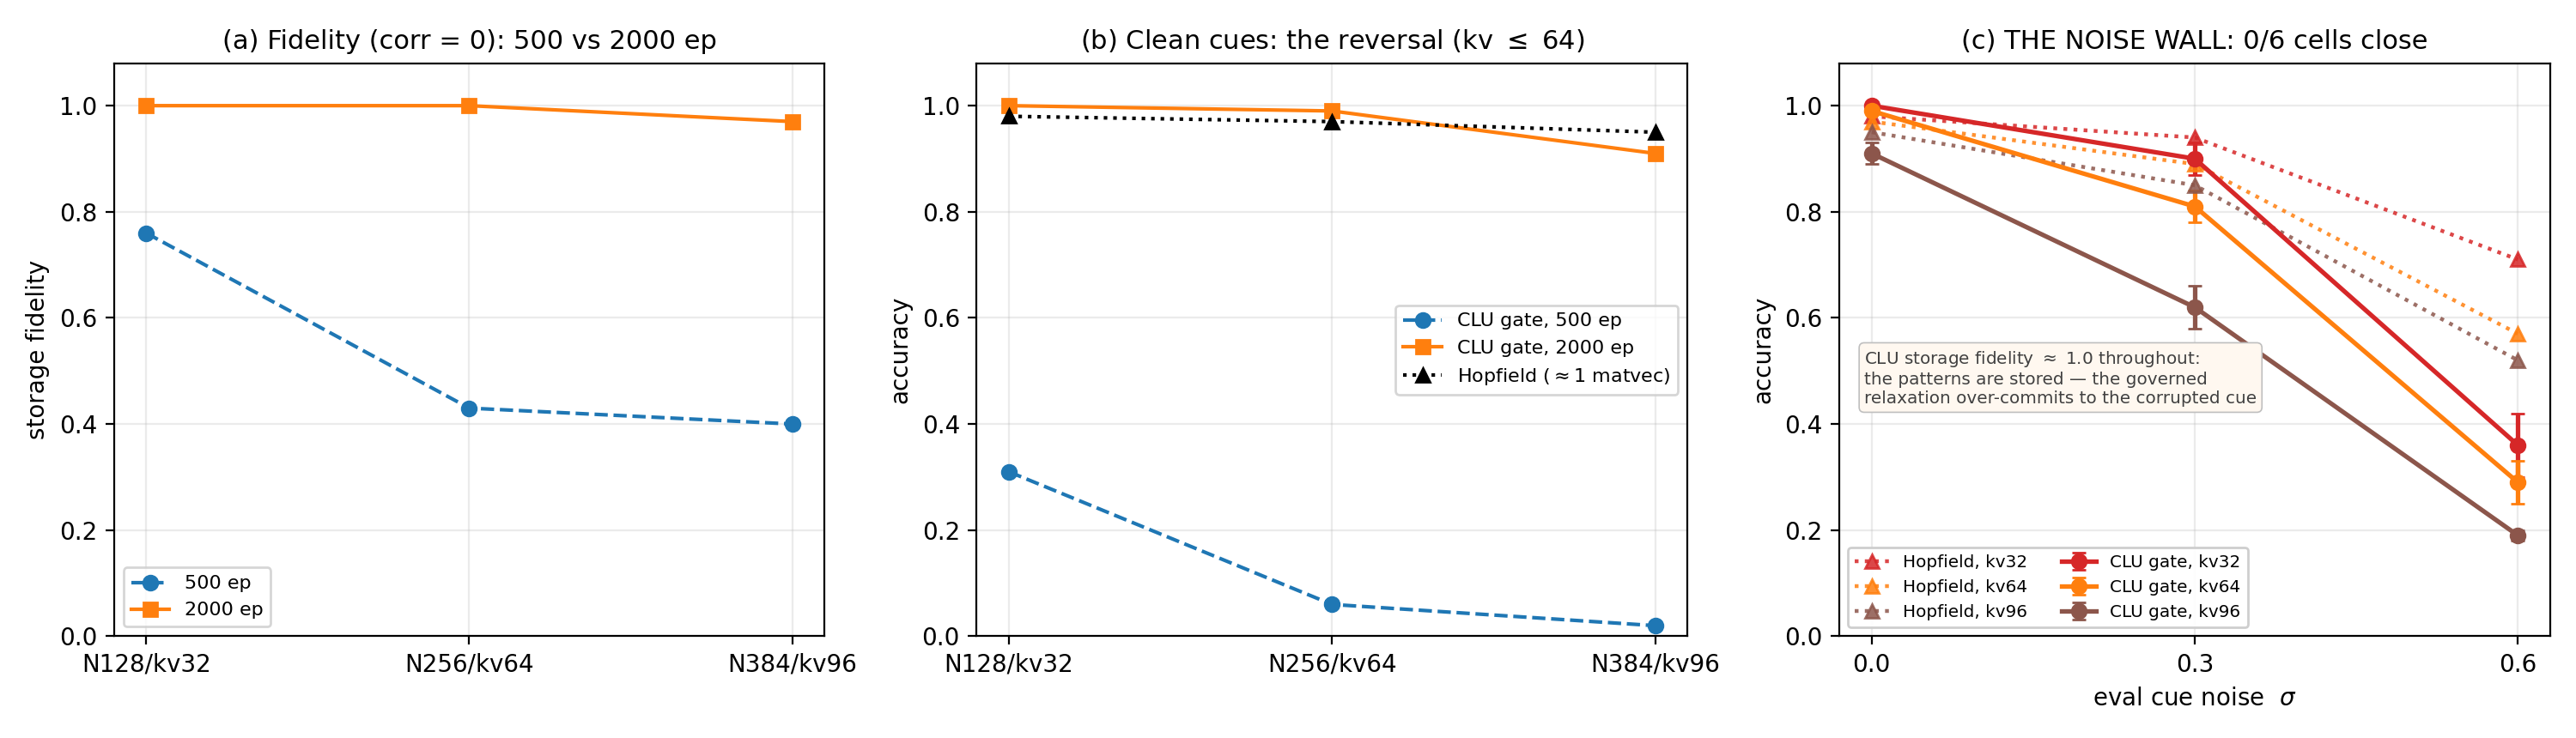
\includegraphics[width=\textwidth]{fig2_regime_map.png}
\caption{\textbf{The settled regime map (\S4.3, evidence; \texttt{regime-remap-2000ep}, $198$ jobs).} \emph{(a)} Storage fidelity on the paired capacity axis, $500$ vs $2000$ ep ($n{=}8$): the $500$-ep ``Hopfield-dominant'' map was an under-training artifact. \emph{(b)} Clean cues: at $2000$ ep the gate reaches/reverses Hopfield for kv$\le64$ ($\Delta+0.02$) at $9$--$10\times$ \emph{intra-CLU} rationing (never a cost win over Hopfield, which answers in $\approx1$ matvec). \emph{(c)} \textbf{The noise wall --- the dominant negative, plotted.} Under eval cue noise $\sigma\in\{0.3,0.6\}$ the gate (solid) falls below Hopfield (dotted) at every capacity --- $0/6$ cells close --- \emph{despite} CLU storage fidelity $\approx1.0$: the patterns are stored, but the governed relaxation over-commits to the corrupted cue. Error bars are $\pm1$ s.d.\ over seeds for the gate ($n{=}5$ at $\sigma>0$; $n{=}8$ at the $\sigma{=}0$ clean reference, taken from the corr$=0$ capacity axis); the source reports no per-seed spread for the stress-axis Hopfield arm, so its curves carry no bars.}
\label{fig:regime}
\end{figure}

\begin{figure}[t]\centering

\includegraphics[width=0.72\linewidth]{fig_frontier_clean.png}
\caption{\textbf{Epoch-scaling frontier (\S4.3, evidence).} Gate accuracy and storage fidelity vs training epochs across kv$\in\{32,64,96,128\}$, against the epoch-independent Hopfield band ($0.947$--$0.976$): an epoch-budget ridge, not a capacity wall; kv$32$ over-trains ($1.00\to0.89$). \emph{(Candidate for the appendix at the pruning pass.)}}
\label{fig:frontier}
\end{figure}

\section{Position, scope, and horizon}
\paragraph{The position, restated.} On a conservative memory, test-time compute is \emph{paid access}, and the price list is physical: a squeeze buys escape for a bounded, re-absorbable injection and \textbf{prices reach exponentially} (it exceeds the box only by its instantaneous displacement $p_0\sinh\zeta/M_0$, at energy cost $e^{2\zeta}$); a wormhole buys \textbf{unbounded} reach for a $\detJ=1$ receipt and a \emph{fixed} discrete ledger, and transports rather than destroys stored content --- where an untrained $\detJ=0$ \textbf{state-replacing} jump, which reaches by overwriting the state, provably erases it. (Deciding \emph{whether} to take that certified edge is separate: \S4.2's learned decision head routes \emph{through} the channel and inherits its receipt --- decision and transport are orthogonal.) These are theorems verified to machine precision (\S3), composing with the memory's BIBO guarantees \emph{only under coercive-component screening} --- a bounded, or even free, energy ledger is not enough (App.~B.2). Where a learned halting head or an energy verifier (Gladstone et al.\ 2025) escalates \emph{the same operation} with no structural account, a symplectic memory prices each access mechanism \emph{and certifies what it did to the state}. The honest pillars of \S4 delimit where this buys a real ML advantage (escalatable rationing) and where a cheaper black box wins (routing): a certificate stack is a design discipline, not a guarantee of dominance.

\paragraph{Scope (stated, not buried).} The \S3 verifications use \textbf{oracle channel placement}, dim $2$/$4$, $5$ seeds, laptop-CPU; the \S4 learned-memory pillars are MQAR-style, vocab-$256$, kv/$N$ small, laptop-CPU. No claim here is at scale, and none uses learned placement.

\paragraph{Horizon / future work.}
\begin{itemize}\itemsep1pt
\item \textbf{Learned entrance-steering is the engineering crux.} The reach theorem proves the outer reachable set, but a trajectory must still \emph{arrive} at a channel entrance under the flow; placing/learning $(a,b)$ so entrances sit on natural trajectories is the true cost at scale and the likely failure point --- addressed in forthcoming work.
\item \textbf{Certifying exits on a \emph{learned} potential.} The BIBO receipt (App.~B.2) screens exits against the coercive component of an \emph{analytic} well with closed-form $x_b$. For a learned, architecturally non-coercive $V_\theta$ the boundary is unknown; a sub-level-set estimator (or restoring the $\alpha\|q\|^2$ confinement Deep/Conv drop) is the natural next experiment. Our coercive screen is an oracle, exactly as our channel placement is.
\item \textbf{$\gamma$-re-absorption timing.} The governor re-absorption certificate ($t_{\rm reabsorb}\approx2\zeta/\gamma_c$) is verified only to leading order at $\gamma=0$; a $\gamma>0$ sweep closes that row.
\item \textbf{Retry acceptance as a certified kernel} is developed as the closing design-rules below (derivations in App.~F).
\end{itemize}

\paragraph{Test-time retries as a certified Markov kernel --- four design rules (theory-complete on toy EBMs; no runs on trained CLU checkpoints are claimed).} The paid-access logic extends one level up, from a single access mechanism to the \emph{acceptance rule} governing repeated retries. Because the squeeze $S^{(M)}_\zeta$ is exactly symplectic ($\detJ=1$), a sign-symmetrized squeeze accepted by $\min(1,e^{-\Delta H/T})$ needs \textbf{no Jacobian correction} and is a $\pi$-reversible kernel for the Gibbs measure of the trained energy --- test-time compute as MCMC with a \emph{stationarity certificate} (Duane et al.\ 1987; Neal 2011). Four rules follow, each with its receipt, and each a restriction rather than a promise.
\begin{enumerate}\itemsep1pt
\item \textbf{Run certified segments at $\gamma=0$; keep the governor outside them.} State-dependent $\gamma(H)>0$ is non-$\pi$-preserving dissipation, so the actual squeeze-then-relax cascade is \textbf{Metropolis-within-annealing} toward a colder, MAP-seeking measure ($T_{\rm eff}:1.0\to0.61$ as $\gamma:0\to0.2$, verified) --- possibly \emph{desirable for retrieval}, but \textbf{not Gibbs sampling. We never claim stationarity for the governed composite.}
\item \textbf{Mix; do not rely on the squeeze alone.} The squeeze family is a one-parameter subgroup whose orbit is a single hyperbola, hence \textbf{reducible/non-ergodic}; read it as a mass-metric-preconditioned \emph{reach} move and use $\tfrac12\,\mathrm{MALA}(\sigma^\star)+\tfrac12$ sign-symmetrized squeeze-MH (a mixture of $\pi$-reversible kernels is $\pi$-reversible).
\item \textbf{Calibrate the Langevin noise by fluctuation--dissipation (Newtonian kinetic mode).} The discrete FDT scale $\sigma_i^\star=\sqrt{M_{{\rm eff},i}T\gamma(2-\gamma)}$ is load-bearing, not cosmetic: it moves the sampler from shadow-biased to exact ($L_1$ $0.0995\to0.0065$, float64 toy EBMs). \emph{Scope (a scope clause, not a caveat --- V1's units are Newtonian throughout):} this exactness is a Newtonian-mode statement. Once the step is Metropolis-adjusted, $\sigma^\star$ is a \emph{proposal-tuning} scale (mixing efficiency), not a correctness condition --- any $\sigma$ leaves $\pi$ invariant under MH, and the $0.0995\to0.0065$ gain is the finite-budget shadow bias it removes. In a relativistic kinetic mode the momentum target is Maxwell--J\"uttner, for which a fixed-covariance Gaussian kick is not a Gibbs refresh, so there the MH correction --- not $\sigma^\star$ --- secures stationarity (App.~F.2).
\item \textbf{Project every proposal off the coset tangent --- even the certified retry carries a receipt.} The Gibbs measure is \emph{exactly flat} along the Goldstone coset, so coset-tangent proposals are accepted w.p.\ $1$ and \textbf{random-walk the stored register} at $D=\tfrac12 s^2$, erasing it after $N_{\rm erode}\approx(\Delta_{\rm read}/s)^2$ accepted moves [proven; verified $D=1.29{\times}10^{-3}$ vs $\tfrac12 s^2=1.25{\times}10^{-3}$] --- true even for a \emph{charge}-preserving isotropic squeeze, which conserves $Q$ while eroding coset \emph{position}. Projection quenches it ($D=0$, verified).
\end{enumerate}
Per the energy-is-not-a-signal discipline held throughout: the acceptance temperature that makes the kernel \emph{useful} is a per-model, write-time-calibrated quantity --- the same learned gate \S4.1 already fits --- so \textbf{the value of the MH framing is the stationarity certificate and the explicit erosion accounting, not parameter parsimony, and not, on current evidence, performance}. Derivations, the four numerical checks, and the specified discriminating experiment are in App.~F.

\paragraph{Prior-art honesty.} The nonlocal edge overlaps attention, skip connections, and MoE routing (Shazeer et al.\ 2017; Raposo et al.\ 2024); the squeeze overlaps simulated-annealing / basin-hopping / MCMC proposals; the certified-kernel reading sits in the Hamiltonian-Monte-Carlo (Duane et al.\ 1987; Neal 2011) and Metropolis-adjusted-Langevin (Roberts \& Tweedie 1996) lineage (the squeeze a linear, gradient-free, mass-preconditioned replacement for the leapfrog trajectory; $\sigma^\star$ an FDT calibration, not a new algorithm); the coset-erosion result is Mermin--Wagner-flavoured; and the relativistic cap has a physics precedent in Lieb--Robinson light-cone bounds (Lieb \& Robinson 1972). We cite these for the bound and lineage and claim only the \emph{design consequences} --- the $\detJ=1$ + energy-ledger + latch-transport certificate, and the governor-composed, coset-projected, FDT-calibrated, bounded-injection acceptance with an explicit certified-retry erosion budget --- not novelty of nonlocality, stochastic escape, MCMC itself, or the causal bound.

\appendix
\section{Flag-provenance tables}
All results inherit their exact non-default configuration; see \texttt{draft.md} Appendix~A for the full four tables (\S3 certificate stack, commit \texttt{6f2384c}; \S4.1 gate, commit \texttt{572c708}, with the memory-agnostic Hopfield transfer $0.18\to0.88$ from \texttt{minus-the-physics} Part~B, $5$ seeds; \S4.2 routing, commit \texttt{52330f8}; \S4.3 regime map, commit \texttt{63fea62}, \texttt{regime-remap-2000ep} $198$ jobs, \texttt{train\_epochs}$\in\{500,1000,2000,4000\}$ the swept arm, $n{=}8$ capacity / $n{=}5$ stress / $n{=}3$ frontier; \textbf{\S3.2.1 latch payoff + App.~B.2 BIBO battery, commit \texttt{27f232f}} (\texttt{v1-certificate-payoff}, JAX $0.9.0$, no training, oracle placement, $5$ seeds, dim $2$\,\&\,$4$)). Key non-defaults: \S3 mass band $[4.0,0.25]$, relativistic + Newtonian-control modes, $\gamma=0$ reach rollout, $dt=0.05$, $T=100\Rightarrow L=2.5$; App.~B.2 BIBO uses $\gamma=0.02$, $k=1.0$, $\epsilon=0.02\Rightarrow x_b=3.5355$, $V_b=3.125$, $T=2000$ ($r^\ast$ also at $2T$), escape radius $20.0$; \S4 relativistic kinetic, mlp potential, PCD write, \texttt{langevin\_noise=legacy}. Cross-section note (two axes: damping and epochs). \emph{Damping:} \S3's reach rollout uses $\gamma=0$ for a sharp box while App.~B.2 uses $\gamma=0.02$ \emph{because a bounded arm must be able to settle} (at $\gamma=0$ a conservative orbit never converges, so ``bounded'' would be untestable). \emph{Epochs (the axis governing the \S4.1$\leftrightarrow$\S4.3 comparison):} \textbf{\S4.1 trains $400$ ep; \S4.3 sweeps $\{500,1000,2000,4000\}$ ep} --- different budgets, reconciled inline in \S4.1 point 2 (\S4.1's escalatable-accuracy headroom is a $400$-ep, not-yet-converged property; \S4.3 App.~C.4.a gives the converged counterpart, where accuracy \emph{matches} full-budget and the payoff is rationing only).

\section{The paid-access certificate table, and the two fine-print experiments}
\subsection*{B.1\quad Table~1 --- the receipt per mechanism}
\begin{center}\footnotesize
\begin{tabular}{p{2.6cm}p{2.3cm}p{1.8cm}p{3.0cm}p{2.5cm}}
\toprule
mechanism & energy injected (bound) & volume $\detJ$ & governor re-absorption & latch impact \\
\midrule
wormhole (translation) & $\Delta V{=}V(b){-}V(a)$, discrete, ledgered & $\mathbf{1}$ exactly; $(1{-}\gamma)^d$ damped & $\approx(1/\gamma_c)\ln(1{+}\Delta V/E^\star)$ & \textbf{transport}, shift $p^\top X\Delta$ \\
wormhole (throat in $V_\theta$) & standing $\sim A$, no jump & $(1{-}\gamma)^d$ exact & continuous & adds $\mu^2{\propto}A/\ell^2$ \\
squeeze $S^{(M)}$ & $\le(e^{2|\zeta|}{-}1)H$ (matched quad.\ $H$) & $\mathbf{1}$ exactly & $\approx2\zeta/\gamma_c$ & preserved (off-coset) \\
\bottomrule
\end{tabular}
\end{center}
\textbf{BIBO caveat (with the table).} Both compose with a coercive $V_\theta$ and $\gamma>0$ (both $\detJ\le1$). But Deep/Conv potentials are non-coercive out-of-unit; a wormhole exit into a non-coercive region can escape to infinity. \textbf{Design constraint:} exits inside a coercive sub-level \emph{component} (or with $\alpha\|q\|^2$ confinement). This is now \textbf{exercised and measured} (B.2); the \S3.2 reach testbed uses coercive wells, where the constraint is inactive.

\subsection*{B.2\quad The BIBO battery --- a free ledger does not buy boundedness}
\emph{Reporting grade: verification (designed analytic testbed; oracle placement).} Source \texttt{v1-certificate-payoff} \S7.4. We make the architectural non-coercivity of Deep/Conv potentials analytic and controllable with $V=\half kq_0^2-\epsilon q_0^4+\half\,\mathrm{conf}\,\|q_{1:}\|^2$ ($k=1$, $\epsilon=0.02$, conf $=4.0$), coercive \emph{only} inside the connected component $|q_0|<x_b=\sqrt{k/4\epsilon}=3.536$; barrier $V_b=3.125$. Three arms, six exits $b$; $\gamma=0.02$, $T=2000$, relativistic, $5$ seeds; $r^\ast=\max_t\|q_t\|$ measured at $T$ and $2T$.

\begin{center}\small
\begin{tabular}{lcccccc}
\toprule
arm ($r^\ast$ at $2T$) & $b{=}1.0$ & $2.0$ & $3.0$ & $3.6$ & $4.0$ & $5.0$ \\
\midrule
wormhole $+$ receipt (screened) & $1.01$ & $2.01$ & $3.01$ & $\mathbf{0.09}$ & $\mathbf{0.09}$ & $\mathbf{0.09}$ \\
wormhole, receipt ignored (ablation) & $1.01$ & $2.01$ & $3.01$ & $\mathbf{102.13}$ & $\mathbf{103.43}$ & $\mathbf{104.83}$ \\
state-replacing map (no receipt) & $1.01$ & $2.01$ & $3.01$ & $\mathbf{102.13}$ & $\mathbf{103.43}$ & $\mathbf{104.83}$ \\
\midrule
escape rate, certified & $0$ & $0$ & $0$ & $0$ & $0$ & $0$ \\
escape rate, blind / router & $0$ & $0$ & $0$ & $1.0$ & $1.0$ & $1.0$ \\
\textbf{wormhole receipt} & ADMIT & ADMIT & ADMIT & REJECT & REJECT & REJECT \\
\emph{energy-only sub-level test} & admit & admit & admit & reject & \textbf{admit} & \textbf{admit} \\
\bottomrule
\end{tabular}
\end{center}
($T$-values for the escaping arms: $52.12/53.43/54.83$.)

\begin{enumerate}\itemsep1pt
\item \textbf{The diagnostic is a growth rate, not a big number.} $r^\ast(2T)/r^\ast(T)=1.000$ for every bounded arm/exit (saturated) vs $1.96/1.94/1.91$ for the escaping ones --- $r^\ast\propto T$, genuinely unbounded, terminal velocity capped at $c/\sqrt{M_0}=0.5$ by the relativistic governor. \textbf{The causal cap bounds speed, not excursion.}
\item \textbf{The receipt predicts BIBO blow-up on $6/6$ exits}; the ledger $\Delta H=V(b)-V(a)$ is exact to $0.0$ at every exit.
\item \textbf{The killer row is $b=5.0$.} $V(5.0)=0.0$ \emph{exactly}: the ledger says the jump is \textbf{free} --- cheaper than the admissible $b=3.0$ exit ($\Delta H=2.88$) --- and an energy-only sub-level test \textbf{admits} it. It escapes anyway; likewise $b=4.0$ ($V=2.88<V_b$; note $V(3.0)=V(4.0)=2.88$ exactly, a coincidence of $\half x^2-0.02x^4$). \textbf{$\detJ=1$ plus a bounded --- or even zero --- ledger is NOT sufficient for BIBO; coercive-\emph{component} membership is the operative clause.}
\item \textbf{Attribution, honestly.} \texttt{wormhole\_blind} and \texttt{no\_physics\_router} \textbf{coincide exactly}: neither is screened. So what buys BIBO is \textbf{the receipt, not the jump mechanism}. The defensible claim: \emph{the wormhole can form the receipt} (it has $V_\theta$, an exact ledger, a well-defined Jacobian) \emph{and a physics-free state-replacing map has none of the three and cannot screen its own exit even in principle} --- bolting a coercivity check onto it means handing it the certificate machinery. \textbf{Payoff A (\S3.2.1) carries no such caveat, which is why it, not this, is the headline panel.}
\item \textbf{The trade the certificate makes explicit.} On rejected exits the certified wormhole \textbf{does not reach the target} ($r^\ast=0.09$; it stays home). The receipt does not make an unsafe exit safe --- it \emph{refuses} it.
\item \textbf{Scope.} The coercive screen uses the analytic $x_b$: an \textbf{oracle} too. Certifying exits on a trained, non-coercive $V_\theta$ is genuinely open. Also $b=3.6$ sits $0.06$ outside $x_b$, yet $r^\ast(2T)=102$ vs $0.09$ and growth $1.96$ make the classification unambiguous --- no knife-edge, unlike the \S3.2 squeeze bracket.
\end{enumerate}

\begin{figure}[t]\centering

\includegraphics[width=0.68\linewidth]{fig4_bibo.png}
\caption{\textbf{BIBO battery (App.~B.2, verification grade).} An uncertified exit escapes ($r^\ast\propto T$); the receipt-screened exit stays bounded by \emph{refusing} to jump. The router curve coincides \emph{exactly} with the receipt-ignored wormhole ablation (drawn as a translucent band under a dashed overlay so neither is occluded) --- the honest reading is that the \emph{receipt}, not the jump, buys boundedness. Note $b=5.0$: the energy ledger is free ($\Delta H=0$) and the exit still escapes.}
\label{fig:bibo}
\end{figure}

\section{Full honest tables}
See \texttt{draft.md} Appendix~C for: (C.1) the full reach battery grid + per-arm certificates (wormhole $\detJ=[1.0]{\times}6$ exact, ledger err $[0.0]{\times}6$; \textbf{state-replacing map (\texttt{no\_physics\_router}) $\detJ=[0.0]{\times}6$, measured by forward-mode autodiff --- volume-annihilating and non-invertible, not merely uncertified}; squeeze $\det S^{(M)}=1.000\pm4\mathrm{e}{-6}$; forbidden state-dependent gate $\detJ=2.05$) and (C.1.b) the latch-payoff cloud for all four arms with replication across dim $\in\{2,4\}\times$ seed $\in\{0,7\}$; (C.2) the routing grid ($N\in\{4,8\}$, all arms, FLOP/query --- router $1.000/0.948$ @ $8.81\mathrm{e}7$ vs gated $0.887/0.715$ @ $1.18\mathrm{e}8$; chain $1.76\mathrm{e}8\to2.94\mathrm{e}8$); (C.3) Hopfield iteration parity (ceiling in $1$ matvec at $\beta\ge5$); (C.4) the settled full-grid regime map --- (C.4.a) paired capacity axis $500$ vs $2000$ ep ($n{=}8$: kv$32$/kv$64$ reverse $\Delta+0.02$, kv$96$ $\Delta-0.04$), (C.4.b) epoch-scaling frontier ($4000$ ep closes kv$96$ $+0.03$, kv$128$ ties; kv$32$ over-trains $1.00\to0.89$), (C.4.c) stress axes including \textbf{the noise wall} (eval-noise $0/6$ close: gate $0.36$ vs Hopfield $0.71$ at $\sigma{=}0.6$/kv$32$ despite fidelity $\approx1.0$) and the $\rho=0.9$ Hopfield-collapse artifact. Tally $6/15$ close at $2000$ ep.

\section{Negatives on the record}
Tier-A V1 negatives (future-work anchors, not hidden failures): \textbf{N1} squeeze retries recover nothing at single-unit scale --- \emph{tested selection among reachable, not crossing to unreachable}; does not bear on \S3 (\S3.3). \textbf{N2} abstention-vs-Hopfield unwinnable; Hopfield dominant at $500$ ep (\emph{provisional --- under-trained map}). \textbf{N3} CLU energy $\approx$ readout margin ($\Delta$AUROC $\in[-0.004,+0.024]$) --- \emph{the forbidden energy-superiority claim, not made}. \textbf{N24} energy-gated wormhole loses to a physics-free router (the \S4.2 boundary). \textbf{N30} $V(\text{data})$-anchor does not transfer to memory fidelity. \textbf{N31} state-dependent jump-gate breaks volume by $\nabla g\cdot\Delta$ ($\detJ=2.05$; the frozen-gate design guard). \textbf{N23} smooth $z$-gate mis-routes $\sim10$--$12\%$. Scope caveat: N24/N27 rest on a linearly-separable-cue laptop testbed --- honest for the tested regime, not proven universal.

\textbf{Fine print of Payoff A --- volume preservation alone is \emph{not} the latch receipt (measured design guard).} The random-shift arm is symplectic ($\detJ=1$) and \emph{still} scrambles the Goldstone charge ($\Delta Q$ std $0.2465$; out-spread $0.2793=3.48\times$ the incoming spread). Only the \textbf{matched channel} ($\Delta$ coset-tangent, $X\Delta\perp p$) makes $\Delta Q$ constant and preserves the spread. Any reading of \S3.2.1 as ``$\detJ=1\Rightarrow$ memory is safe'' is wrong, and we flag it so the fine print cannot be inverted into the review.

\textbf{Fine print of Payoff B --- the receipt buys BIBO, \emph{not} the jump; and the state-replacing map $\equiv$ a blind wormhole.} The \texttt{wormhole\_blind} and \texttt{no\_physics\_router} (state-replacing) arms coincide exactly on all six exits, so no boundedness advantage attaches to the wormhole's jump mechanism per se --- only to the screening receipt, which a physics-free state-replacing map cannot form (no $V_\theta$, no ledger, no Jacobian). And a \textbf{free} ledger ($\Delta H=0$ at $b=5.0$) is admitted by an energy-only test and escapes anyway. This is why the latch (Payoff A), not BIBO (Payoff B), is the headline panel.

\textbf{Payoff scope.} Both payoffs are on the designed testbed: oracle channel placement, analytic potentials, no training. They demonstrate the certificate's \emph{downstream consequence}; they do \textbf{not} claim a real-data or learned-memory win. The coercive screen itself uses the analytic $x_b$ and is likewise an oracle.

\section{Analytic verifications}
\texttt{checks.py}, numpy float64, seed 0; double well $V=\beta(q^2-a^2)^2$, $a=\beta=1$, $\varepsilon=0.05$. (A) reach cap $|\Delta q|=T\varepsilon c/\sqrt{M}$ to rel.\ err $2.0\mathrm{e}{-12}$; (B) plain trapped $q=-1.068$, wormhole $q=+1.000$, ledger $0.0$; (C) $\detJ$ const $=1.000$, state-dep matches $1+\nabla g\cdot\Delta$ to $2.2\mathrm{e}{-16}$; (D) squeeze hop threshold $\zeta^\star=0.2356$ vs measured $0.27$; (E) latch transit err $1.8\mathrm{e}{-15}$, $X\Delta\perp p$ shift $0.0$; (F) re-absorption $56$ vs predicted $49.5$ steps, injection $E_{\rm inj}/E^\star=2.718=e^{2\cdot0.5}$.

\section{Test-time retries as a certified Markov kernel (derivations, checks, specified experiment)}
Source: \texttt{thread9-mh-kernel} ($4$ numerical checks, float64, toy EBMs). \textbf{Grade: theory-complete on toy EBMs. No runs on trained CLU checkpoints are claimed anywhere in this paper.} This appendix carries the derivation behind the four design rules of \S5.

\paragraph{F.1 Why the squeeze needs no Jacobian correction.} $S^{(M)}_\zeta$ is exactly volume-preserving ($\detJ=1$) --- the property HMC (Duane et al.\ 1987; Neal 2011) exploits to avoid a Jacobian correction in the acceptance ratio. A retry proposing a \textbf{sign-symmetrized} squeeze ($\pm\zeta$ with equal probability, restoring proposal symmetry) and accepting with $\min(1,e^{-\Delta H/T})$ is a \textbf{detailed-balance kernel for $e^{-H/T}$} --- test-time compute as MCMC with a stationarity certificate. $\pi$-reversibility is proven and verified ($L_1=0.0095$ between forward and reversed two-step histograms). The certificate is \textbf{narrower than the retry-cascade pitch assumes}; three physics facts sharpen it.

\paragraph{F.2 (i) Squeeze-only is non-ergodic; MALA supplies mixing, FDT supplies its scale.} $\{S_\zeta\}$ is a one-parameter subgroup whose orbit of any point is a \textbf{single hyperbola} in $(q_i,p_i)$: squeeze-only proposals are \textbf{reducible/non-ergodic} and cannot reach off-hyperbola states at all. Ergodicity requires HMC-style momentum refreshment; the squeeze is best read as a \textbf{mass-metric-preconditioned global (reach) move} layered on a MALA step (Roberts \& Tweedie 1996). Its noise scale is not free: the discrete fluctuation--dissipation relation for the damped Verlet step fixes $\sigma_i^\star=\sqrt{M_{{\rm eff},i}\,T\,\gamma(2-\gamma)}$, and this is \textbf{load-bearing rather than cosmetic} --- the FDT-correct $\sigma^\star$ moves the sampler from shadow-biased to exact, $L_1$ error $0.0995\to0.0065$ ($15\times$; float64). \textbf{Kinetic-mode scope (Newtonian only; a scope clause, not a retraction --- V1's units are Newtonian):} (a) once Metropolis-adjusted, $\sigma^\star$ is a proposal-tuning scale (mixing efficiency), not a correctness condition --- any $\sigma$ leaves $\pi$ invariant, and the $0.0995\to0.0065$ gain is the finite-budget shadow bias removed; (b) the Gaussian FDT kick is a Gibbs momentum-refresh only in the Newtonian modes, where $\pi_p$ is Gaussian --- in a relativistic mode $\pi_p$ is Maxwell--J\"uttner, a fixed-covariance Gaussian refresh is not one of its refreshes, and stationarity is secured by the MH correction rather than by any $\sigma^\star$. A mixture of two $\pi$-reversible kernels is $\pi$-reversible, so $\half\mathrm{MALA}(\sigma^\star)+\half$ squeeze-MH inherits the certificate.

\paragraph{F.3 (ii) The governor destroys the invariant: the real cascade is annealing, not sampling.} State-dependent $\gamma(H)>0$ is non-$\pi$-preserving dissipation, so the deployed squeeze-then-relax cascade is \textbf{Metropolis-within-annealing}, converging to a colder MAP-seeking measure: $T_{\rm eff}:1.0\to0.61$ as $\gamma:0\to0.2$ (verified, float64). This may be \emph{desirable for retrieval} --- a MAP-seeking cascade is what an associative memory wants --- but \textbf{it is not Gibbs sampling, and we never claim stationarity for the governed composite.} Hence design rule 1.

\paragraph{F.4 (iii) Decisive for a memory: even the certified retry erodes the latch.} The Gibbs measure is \textbf{exactly flat along the Goldstone coset} (no restoring force along a broken continuous symmetry), so any coset-tangent proposal has $\Delta H=0$ and is accepted w.p.\ $1$. Accepted coset-tangent moves compose into an unbiased random walk that \textbf{diffuses the stored register} at $D=\half s^2$ per accepted move, with $N_{\rm erode}\approx(\Delta_{\rm read}/s)^2$, where $s$ is the proposal scale and $\Delta_{\rm read}$ the read-out margin along the coset [proven; verified $D=1.29{\times}10^{-3}$ vs $\half s^2=1.25{\times}10^{-3}$]. This holds \textbf{even for a \emph{charge}-preserving isotropic squeeze}, which conserves $Q=p^\top Xq$ while eroding coset \emph{position} --- charge and position are different observables and only the former is protected. Projecting proposals off the coset tangent quenches it ($D=0$, verified), so only explicit writes move the register.

\paragraph{F.5 The deflation we state rather than bury.} Acceptance is an \emph{intra-model} quantity: cross-model incomparability of $H$ does not break validity, but the operating temperature $T$ that makes the kernel \emph{useful} is model-specific and FDT-miscalibrated in general. A per-model $T$ therefore \textbf{partially re-imports the learned gate} of \S4.1 --- the parsimony argument is weak. \textbf{The value of the MH framing is the stationarity certificate and the explicit erosion accounting, not parameter parsimony, and not, on current evidence, performance.}

\paragraph{F.6 The specified discriminating experiment (future work).} Three arms (certified mixture kernel at $\gamma=0$ with coset projection; the learned-$\tau$ escalation gate of \S4.1; naive squeeze retries) on a trained CLU associative memory, matched on FLOPs, with \textbf{the latch-erosion decay curve as the money plot} --- predicting that naive certified retries erode the register at $D=\half s^2$ while the coset-projected kernel holds it flat. Risks: (a) the erosion rate is derived on toy EBMs and a trained-$V_\theta$ coset is only approximately flat; (b) the FDT $\sigma^\star$ assumes the damped-Verlet noise model, which \texttt{langevin\_noise=legacy} runs violate; (c) matched-FLOPs accounting must charge the MALA gradient. \textbf{Not run; no CLU-checkpoint result is claimed.}

\section*{References}
\small
\begin{itemize}\itemsep0pt
\item Angelopoulos, A.~N., Bates, S., et al.\ (2021). \emph{Learn then Test: Calibrating Predictive Algorithms to Achieve Risk Control.}
\item Banino, A., Balaguer, J., Blundell, C.\ (2021). \emph{PonderNet: Learning to Ponder.}
\item Duane, S., Kennedy, A.~D., Pendleton, B.~J., Roweth, D.\ (1987). \emph{Hybrid Monte Carlo.} Physics Letters B.
\item Geifman, Y., El-Yaniv, R.\ (2017). \emph{Selective Classification for Deep Neural Networks.} NeurIPS.
\item Gladstone, A., et al.\ (2025). \emph{Energy-Based Transformers are Scalable Learners and Thinkers.} arXiv:2507.02092. (preprint; venue status unverified.)
\item Graves, A.\ (2016). \emph{Adaptive Computation Time for Recurrent Neural Networks.} arXiv:1603.08983.
\item Jawahar, P., Pierini, M.\ (2026). \emph{[CHLU primitive --- the CLU is introduced as CHLU here].}
\item Lieb, E.~H., Robinson, D.~W.\ (1972). \emph{The Finite Group Velocity of Quantum Spin Systems.} Comm.\ Math.\ Phys.
\item Neal, R.~M.\ (2011). \emph{MCMC using Hamiltonian dynamics.} Handbook of MCMC.
\item Platt, J.\ (1999). \emph{Probabilistic Outputs for Support Vector Machines.}
\item Ramsauer, H., et al.\ (2021). \emph{Hopfield Networks is All You Need.} ICLR.
\item Raposo, D., et al.\ (2024). \emph{Mixture-of-Depths.} arXiv:2404.02258.
\item Roberts, G. O., Tweedie, R. L.\ (1996). \emph{Exponential Convergence of Langevin Distributions and Their Discrete Approximations.} Bernoulli.
\item Schuster, T., et al.\ (2022). \emph{Confident Adaptive Language Modeling.} NeurIPS.
\item Shazeer, N., et al.\ (2017). \emph{Outrageously Large Neural Networks: The Sparsely-Gated MoE Layer.} ICLR.
\item Wales, D.~J., Doye, J.~P.~K.\ (1997). \emph{Global Optimization by Basin-Hopping.} J.\ Phys.\ Chem.\ A.
\item Anonymous (2026). \emph{[The theory note --- exactly-solvable damped-symplectic memory; third person per hermetic-citation policy].}
\end{itemize}

\end{document}
